\chapter{程序计数器 PC 与地址寄存器 AR 实验}
\section{实验内容}

设计 PC 与 AR,采用两种不同的连线方式。

\begin{enumerate}
    \item 总线开关式
    \item 三态门式
\end{enumerate}

\section{实验原理}

\subsection{多路总线开关式}

\begin{figure}[H]
\centering
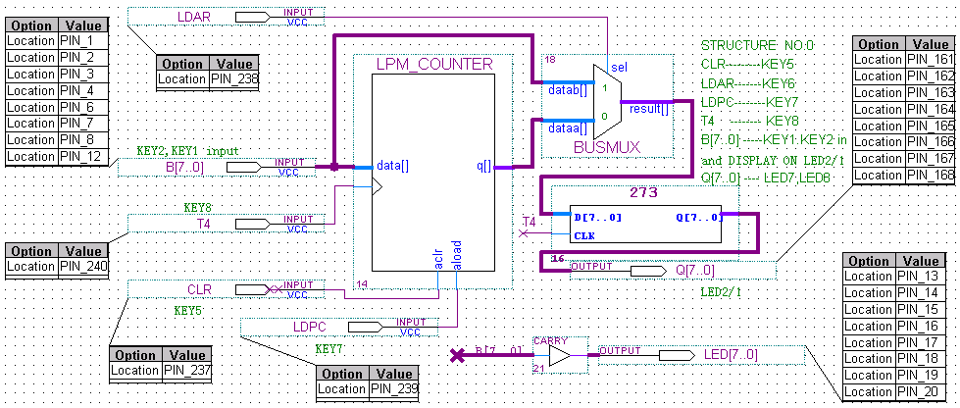
\includegraphics[width=\textwidth]{images/prin4_1.png}
\caption{PC \& AR 实验 总线开关式 原理图}
\label{fig:prin4_1}
\end{figure}

如图\ref{fig:prin4_1},由LPM\_COUNTER, BUSMUX 2 路总线开关,273 寄存器 (AR) 组成,数据线 8 位。

\subsubsection{输入信号}

\begin{itemize}
    \item T4
    
    时钟脉冲信号。

    可由外部控制的输入信号。
    
    \item B[7..0]
    
    数据总线信号,8 位,用于输入指令。
    
    可由外部控制的输入信号。
    
    \item LDAR
    
    控制信号,是否启用 B 信号。0: 禁用,1: 启用。
    
    可由外部控制的输入信号。
    
    \item CLR
    
    控制信号,清空 LPM\_COUNTER 的值。0: 不清零,1: 清零。
    
    可由外部控制的输入信号。
    
    \item LDPC
    
    控制信号,控制 LPM\_COUNTER 是否从 data 端装入数据。0: 不装入,1: 装入。
    
    可由外部控制的输入信号。
    
\end{itemize} 

\subsubsection{输出信号}

\begin{itemize}
    \item Q[7..0]
    
    显示地址寄存器输出的数据,8 位。
    
    \item LED[7..0]
    
    显示 B[7..0] 输入信号,8 位。
    
\end{itemize}

\subsection{三态门式}

\begin{figure}[H]
\centering
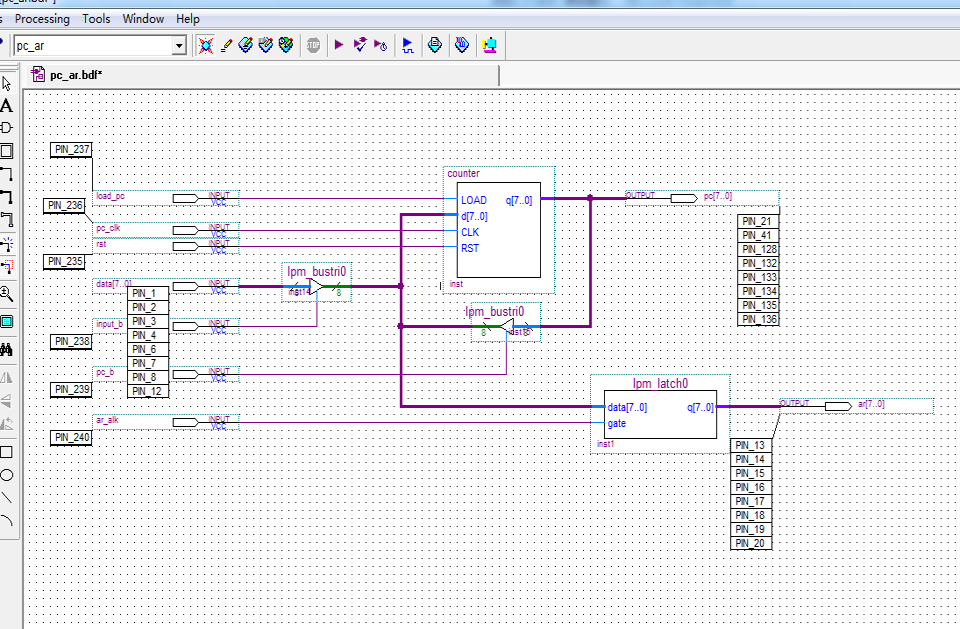
\includegraphics[width=\textwidth]{images/prin4_2.png}
\caption{PC \& AR 实验 三态门式 原理图}
\label{fig:prin4_2}
\end{figure}

如图\ref{fig:prin4_2},由LPM\_COUNTER, lpm\_bustri0 三态门,latch锁存器组成,数据线 8 位。

\subsubsection{输入信号}

\begin{itemize}
    \item pc\_clk
    
    时钟脉冲信号,其上升沿时计数器自增 1。

    可由外部控制的输入信号。
    
    \item data[7..0]
    
    数据总线信号,8 位,用于输入指令。
    
    可由外部控制的输入信号。
    
    \item load\_pc
    
    控制信号,控制计数器从其 d 端加载数据。0: 不加载,1: 加载。

    可由外部控制的输入信号。
    
    \item rst
    
    控制信号,控制计数器清零。0: 不清零,1: 清零。
    
    可由外部控制的输入信号。

    \item input\_b
    
    控制信号,控制左侧三态门的开闭。0: 闭,1: 开。
    
    可由外部控制的输入信号。
    
    \item ar\_clk
    
    时钟脉冲信号,其上升沿时锁存器从其 data 端加载数据。

    可由外部控制的输入信号。
    
    \item pc\_b

    控制信号,控制右侧三态门的开闭。0: 闭,1: 开。
        
    可由外部控制的输入信号。
    
\end{itemize} 

\subsubsection{输出信号}

\begin{itemize}
    \item pc[7..0]
    
    显示计数器输出的 PC 数据,8 位。
    
    \item ar[7..0]
    
    显示锁存器输出的 AR 数据,8 位。
    
\end{itemize}

\section{实验任务与实验步骤}

\subsection{总线开关式}

\begin{enumerate}
    \item 按照原理图 \ref{fig:prin4_1} 连接电路图,然后编译。
    
    \begin{enumerate}
        \item 创建 LPM\_COUNTER 计数器
        
        \begin{itemize}
            \item 启用异步清除
            \item 启用异步加载
            \item 禁用异步置位
            \item 禁用同步清除
            \item 禁用同步加载
            \item 禁用同步置位
        \end{itemize}
        
    \end{enumerate}
    
    \item 将输入输出器件绑定到对应的引脚上,然后重新编译。
    
    \begin{table}[H]
        \centering
        \begin{tabular}{|c|c|c|}
            \hline
            名称 & 引脚号 & 备注 \\
            \hline
            CLR & 237 & Key 5 \\
            \hline
            LDAR & 238 & Key 6 \\
            \hline
            LDPC & 239 & Key 7 \\
            \hline
            T4 & 240 & Key 8 \\
            \hline
            B[0] & 1 & Key 1 \\
            \hline
            B[1] & 2 & Key 1 \\
            \hline
            B[2] & 3 & Key 1 \\
            \hline
            B[3] & 4 & Key 1 \\
            \hline
            B[4] & 6 & Key 2 \\
            \hline
            B[5] & 7 & Key 2 \\
            \hline
            B[6] & 8 & Key 2 \\
            \hline
            B[7] & 12 & Key 2 \\
            \hline
            LED[0] & 13 & 数码 1 \\
            \hline
            LED[1] & 14 & 数码 1 \\
            \hline
            LED[2] & 15 & 数码 1 \\
            \hline
            LED[3] & 16 & 数码 1 \\
            \hline
            LED[4] & 17 & 数码 2 \\
            \hline
            LED[5] & 18 & 数码 2 \\
            \hline
            LED[6] & 19 & 数码 2 \\
            \hline
            LED[7] & 20 & 数码 2 \\
            \hline
            Q[0] & 161 & 数码 7 \\
            \hline
            Q[1] & 162 & 数码 7 \\
            \hline
            Q[2] & 163 & 数码 7 \\
            \hline
            Q[3] & 164 & 数码 7 \\
            \hline
            Q[4] & 165 & 数码 8 \\
            \hline
            Q[5] & 166 & 数码 8 \\
            \hline
            Q[6] & 167 & 数码 8 \\
            \hline
            Q[7] & 168 & 数码 8 \\
            \hline
        \end{tabular}
        \caption{PC \& AR 实验:总线开关式引脚表}
        \label{tab:pin4_1}
    \end{table}
    
    
    \item 下载到实验设备上。
    \item 调整为工作模式 0。
    \item 观察实验现象。
    
    \begin{itemize}
        \item Key 1, 2 (D1 - D8)
        
        控制输入数据 B,8 位全有效,同时显示在数码 1 - 2 上。
        
        \item Key 5 (D13)
        
        控制是否清空计数器。
        
        \item Key 6 (D14)
        
        控制是否加载 AR。
        
        \item Key 7 (D15)
        
        控制是否加载 PC。
        
        \item Key 8 (D16)
        
        控制时钟。
        
        \item 数码管 1, 2
        
        显示输入数据 B 的值,8 位全有效。
        
        \item 数码管 7, 8
        
        地址寄存器 AR 输出的值,8 位全有效。
        
    \end{itemize}
    \item 绘制仿真波形图。
\end{enumerate}

\subsection{三态门式}

\begin{enumerate}
    \item 按照原理图 \ref{fig:prin4_2} 连接电路图,然后编译。

    \begin{enumerate}
        \item 创建 LPM\_COUNTER 计数器
        
        \begin{itemize}
            \item 启用异步清除
            \item 禁用异步加载
            \item 禁用异步置位
            \item 禁用同步清除
            \item 启用同步加载
            \item 禁用同步置位
        \end{itemize}
        
    \end{enumerate}

    
    \item 将输入输出器件绑定到对应的引脚上,然后重新编译。
    
    \begin{table}[H]
        \centering
        \begin{tabular}{|c|c|c|}
            \hline
            名称 & 引脚号 & 备注 \\
            \hline
            rst & 235 & Key 3 \\
            \hline
            pc\_clk & 236 & Key 4 \\
            \hline
            load\_pc & 237 & Key 5 \\
            \hline
            input\_b & 238 & Key 6 \\
            \hline
            pc\_b & 239 & Key 7 \\
            \hline
            ar\_clk & 240 & Key 8 \\
            \hline
            data[0] & 1 & Key 1 \\
            \hline
            data[1] & 2 & Key 1 \\
            \hline
            data[2] & 3 & Key 1 \\
            \hline
            data[3] & 4 & Key 1 \\
            \hline
            data[4] & 6 & Key 2 \\
            \hline
            data[5] & 7 & Key 2 \\
            \hline
            data[6] & 8 & Key 2 \\
            \hline
            data[7] & 12 & Key 2 \\
            \hline
            ar[0] & 13 & 数码 1 \\
            \hline
            ar[1] & 14 & 数码 1 \\
            \hline
            ar[2] & 15 & 数码 1 \\
            \hline
            ar[3] & 16 & 数码 1 \\
            \hline
            ar[4] & 17 & 数码 2 \\
            \hline
            ar[5] & 18 & 数码 2 \\
            \hline
            ar[6] & 19 & 数码 2 \\
            \hline
            ar[7] & 20 & 数码 2 \\
            \hline
            pc[0] & 21 & 数码 3 \\
            \hline
            pc[1] & 41 & 数码 3 \\
            \hline
            pc[2] & 128 & 数码 3 \\
            \hline
            pc[3] & 132 & 数码 3 \\
            \hline
            pc[4] & 133 & 数码 4 \\
            \hline
            pc[5] & 134 & 数码 4 \\
            \hline
            pc[6] & 135 & 数码 4 \\
            \hline
            pc[7] & 136 & 数码 4 \\
            \hline
        \end{tabular}
        \caption{PC \& AR 实验:三态门式引脚表}
        \label{tab:pin4_2}
    \end{table}
    
    
    \item 下载到实验设备上。
    \item 调整为工作模式 0。
    \item 观察实验现象。
    
    \begin{itemize}
        \item Key 1, 2 (D1 - D8)
        
        控制输入数据 B,8 位全有效。
        
        \item Key 3 (D11)
        
        控制是否清空计数器。
        
        \item Key 4 (D12)
        
        控制计数器自增 1。
        
        \item Key 5 (D13)
        
        控制 PC 预置值加载。
        
        \item Key 6 (D14)
        
        控制输入数据 data 对总线的控制权。
        
        把控左侧三态门的开闭。
        
        \item Key 7 (D15)
        
        控制计数器的输出对总线的控制权。

        把控右侧三态门的开闭。
        
        \item Key 8 (D16)
        
        控制锁存器的时钟。
        
        \item 数码管 1, 2
        
        显示锁存器输出的 AR 的数据,8 位全有效。
        
        \item 数码管 3, 4
        
        显示计数器输出的 PC 的数据,8 位全有效。
        
    \end{itemize}
    \item 绘制仿真波形图。
\end{enumerate}


\section{实验结果分析}

\subsection{实验电路图}

根据原理图 \ref{fig:prin4_1} 绘制实验电路图 \ref{fig:bdf4_1}。

\begin{figure}[H]
\centering
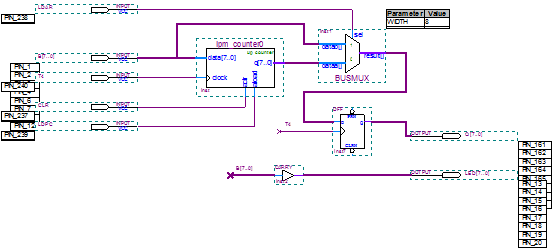
\includegraphics[width=\textwidth]{images/bdf4_1.png}
\caption{PC \& AR 实验 总线开关式 电路图}
\label{fig:bdf4_1}
\end{figure}

根据原理图 \ref{fig:prin4_2} 绘制实验电路图 \ref{fig:bdf4_2}。

\begin{figure}[H]
\centering
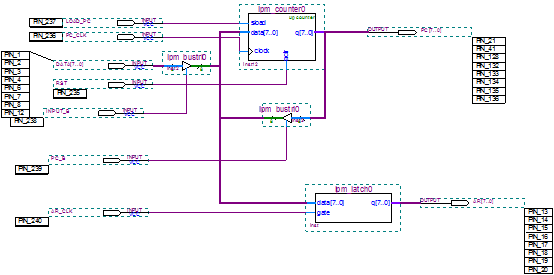
\includegraphics[width=\textwidth]{images/bdf4_2.png}
\caption{PC \& AR 实验 三态门式 电路图}
\label{fig:bdf4_2}
\end{figure}

\subsection{仿真波形图}

利用 Quartus II 产生仿真波形图 \ref{fig:wave4_1}。

\begin{figure}[H]
\centering
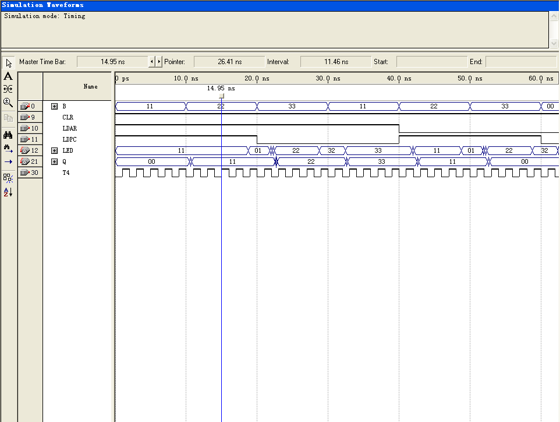
\includegraphics[width=\textwidth]{images/wave4_1.png}
\caption{PC \& AR 实验 总线开关式 仿真波形图}
\label{fig:wave4_1}
\end{figure}

利用 Quartus II 产生仿真波形图 \ref{fig:wave4_2}。

\begin{figure}[H]
\centering
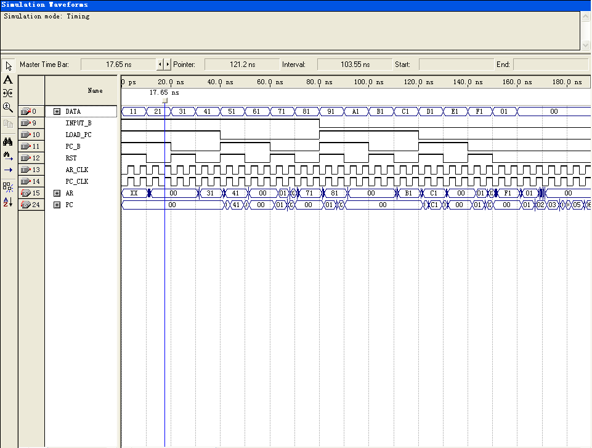
\includegraphics[width=\textwidth]{images/wave4_2.png}
\caption{PC \& AR 实验 三态门式 仿真波形图}
\label{fig:wave4_2}
\end{figure}


\subsection{思考题}

\textbf{声明}:下述题目的回答默认参考三态门式原理图 \ref{fig:prin4_2}:

\begin{enumerate}
    \item 说明顺序执行程序时,将 PC 值送 AR,从 AR 所指向的 RAM 地址单元取出指令的操作。
    
    \textbf{答}:
    
    不包含跳转指令时,PC 的改变始终来源自增 1 的时钟正脉冲信号,全程关闭左侧三态门。

    input\_b := 0 (Key 6)
        
    \begin{enumerate}
        \item 打开右侧三态门,PC 进入内部总线
        
        pc\_b := 1 (Key 7)

        \item 发出锁存器时钟正脉冲,PC $\to$ AR
        
        ar\_clk := 1 (Key 8)
        
        ar\_clk := 0 (Key 8)
        
        \item AR $\to$ Address Bus
        
        这是外部过程。
        
        \item Address Bus $\to$ RAM
        
        这是外部过程。
        
        \item 发出计数器时钟正脉冲,PC := PC + 1
        
        pc\_clk := 1 (Key 4)
        
        pc\_clk := 0 (Key 4)
        
        \item 重复上述操作。
        
    \end{enumerate}
    
    \item 执行分支/转移程序与执行顺序程序时,对地址单元的操作有何区别?
    
    \textbf{答}:
    
    两个三态门的开闭状态不同。
    
    \begin{enumerate}
        \item 分支/转移

        打开左侧三态门,关闭右侧三态门。
        
        \item 顺序执行

        关闭左侧三态门,打开右侧三态门。        
        
    \end{enumerate}
    
    \item 请说明实现 PC 值自动加 1,指向下一个地址单元的操作过程。

    \textbf{答}:
    
    给 pc\_clk 接上指令结束的外部同步脉冲信号 \footnote{这里指 CPU 完成指令后发送的指令结束正脉冲信号} 即可实现 PC 的自动自增 1。
    
    \item 请说明在教材中图 4-65 \footnote{教材图 4-63 为三态门式原理图 \ref{fig:prin4_2}。} 电路中,在实行程序转移时,从 DATA[7..0] 输入转移地址送 PC 和 AR,AR 输出新的转移地址的操作过程。
    
    \textbf{答}:
    
    \begin{enumerate}
        \item 调整内部总线的控制权
        
        \begin{itemize}
            \item 关闭计数器输出对内部总线的控制权开关 PC\_B
            
            PC\_B := 0
            
            \item 打开数据线对内部总线的控制权开关 LOAD\_PC
            
            LOAD\_PC := 1
            
        \end{itemize}
        
        以上两项可并发,均执行完毕后进入下一步。
        
        \item 发送时钟正脉冲信号
        
        \begin{itemize}
            \item 锁存器时钟
            
            AR\_CLK := 0
            AR\_CLK := 1
            
            执行完毕后 AR 应已输出。
            
            \item 计数器时钟
            
            PC\_CLK := 0
            PC\_CLK := 1

            执行完毕后 PC 应已输出。
            
        \end{itemize}
        
        以上两组脉冲可并发。
        
    \end{enumerate}
    
    \item 要实现程序的分支转移,需对教材中图 4-63 \footnote{教材图 4-63 为总线控制式原理图 \ref{fig:prin4_1}。} 中的程序计数器 PC 和地址寄存器 AR 做怎样的操作?应改变那些控制信号?
    
    \textbf{答}:
    
    需要将数据线的值送 PC,然后将 PC 的值送 AR,同时 PC 自增 1。
    
    调整执行顺序如下,可以提高并发性。
    
    \begin{enumerate}
        \item 以下两个操作具有并发性
        
        \begin{itemize}
            \item 送 AR:调整总线选择器 LDAR
            
            LDAR := 1
            
            \item 送 PC:发送时钟正脉冲信号 LDPC
            
            LDPC := 1
            
            defer \footnote{defer: 可延迟执行} LDPC := 0
            
            此时 PC 应已收到数据,但没有输出。
            
        \end{itemize}

        \item 送 AR:发送时钟正脉冲信号 T4
        
        T4 := 1
        
        T4 := 0
        
        此时 AR 已收到数据并输出到 Q,PC 自增 1。
        
    \end{enumerate}
    
    \item 从存储器读取运算数据和执行取指令操作时,地址控制单元完成的操作有何不同?
    
    \textbf{答}:
    
    \begin{itemize}
        \item 从储存器读取运算数据
        
        读操作数发生在指令译码之后,并没有执行完一条指令,不改变 PC 的值。
        
        DATA 总线传入数据地址,应将数据存入 AR,但不改变 PC 的值。
        
        \begin{enumerate}
            \item 调整内部总线控制权
            
            \begin{itemize}
                \item 启用数据总线对内部总线的控制权 INPUT\_B
                
                INPUT\_B := 1
                
                \item 禁用计数器 PC 对内部总线的控制权 PC\_B
                
                PC\_B := 0
                
            \end{itemize}
            
            以上两个操作可并发。
            
            \item 送 AR:发送时钟正脉冲信号 AR\_CLK
            
            AR\_CLK := 1
            
            AR\_CLK := 0
            
        \end{enumerate}
        
        \item 执行取指令操作 (FI)
        
        取指令操作发生在指令译码之前,从 PC 中读取下一条指令的地址,之后 PC 应自增 1。
        
        DATA 总线上的数据是无效的。
        
        \begin{enumerate}
            \item 调整内部总线控制权
            
            \begin{itemize}
                \item 禁用数据总线对内部总线的控制权 INPUT\_B
                
                INPUT\_B := 0
                
                \item 启用计数器 PC 对内部总线的控制权 PC\_B
                
                PC\_B := 1
                
            \end{itemize}
            
            以上两个操作可并发。
            
            \item PC $\to$ AR:发送时钟正脉冲信号 AR\_CLK
            
            AR\_CLK := 1
            
            AR\_CLK := 0
            
            \item PC := PC + 1:发送时钟正脉冲信号 PC\_CLK
            
            PC\_CLK := 1
            
            PC\_CLK := 0
            
        \end{enumerate}

    \end{itemize}
    
\end{enumerate}
